\documentclass{article}

\usepackage[utf8]{inputenc}
\usepackage{polski}
\usepackage{graphicx}
\usepackage{listings}
\usepackage{color}
\usepackage{xcolor}
\usepackage{mathtools}
\usepackage{lscape}
\usepackage[font=small, labelfont=bf]{caption}
\usepackage[margin=0.45in]{geometry}
\usepackage{pdfpages}

\title{Inżynieria oprogramowania 1 \\Game Project \\Dokumentacja}
\author{Filip Grajek, Kamil Grabowski, Bartosz Jasiński, Ivan Rukhavets}
\date{\today}

\begin{document}
\maketitle
	\begin{titlepage}				
		\center{\Large{\textrm{Wydział Matematyki i Nauk Informacyjnych Politechniki Warszawskiej}}}
		
		\begin{figure}
			\centering
\includegraphics[scale=0.3]{./logo.png}
		\end{figure}		
	
	\end{titlepage}
	
	\tableofcontents


	\newpage
	
%	\section{Use Case'y}


%	\begin{figure}[htbp!]
%\centering
%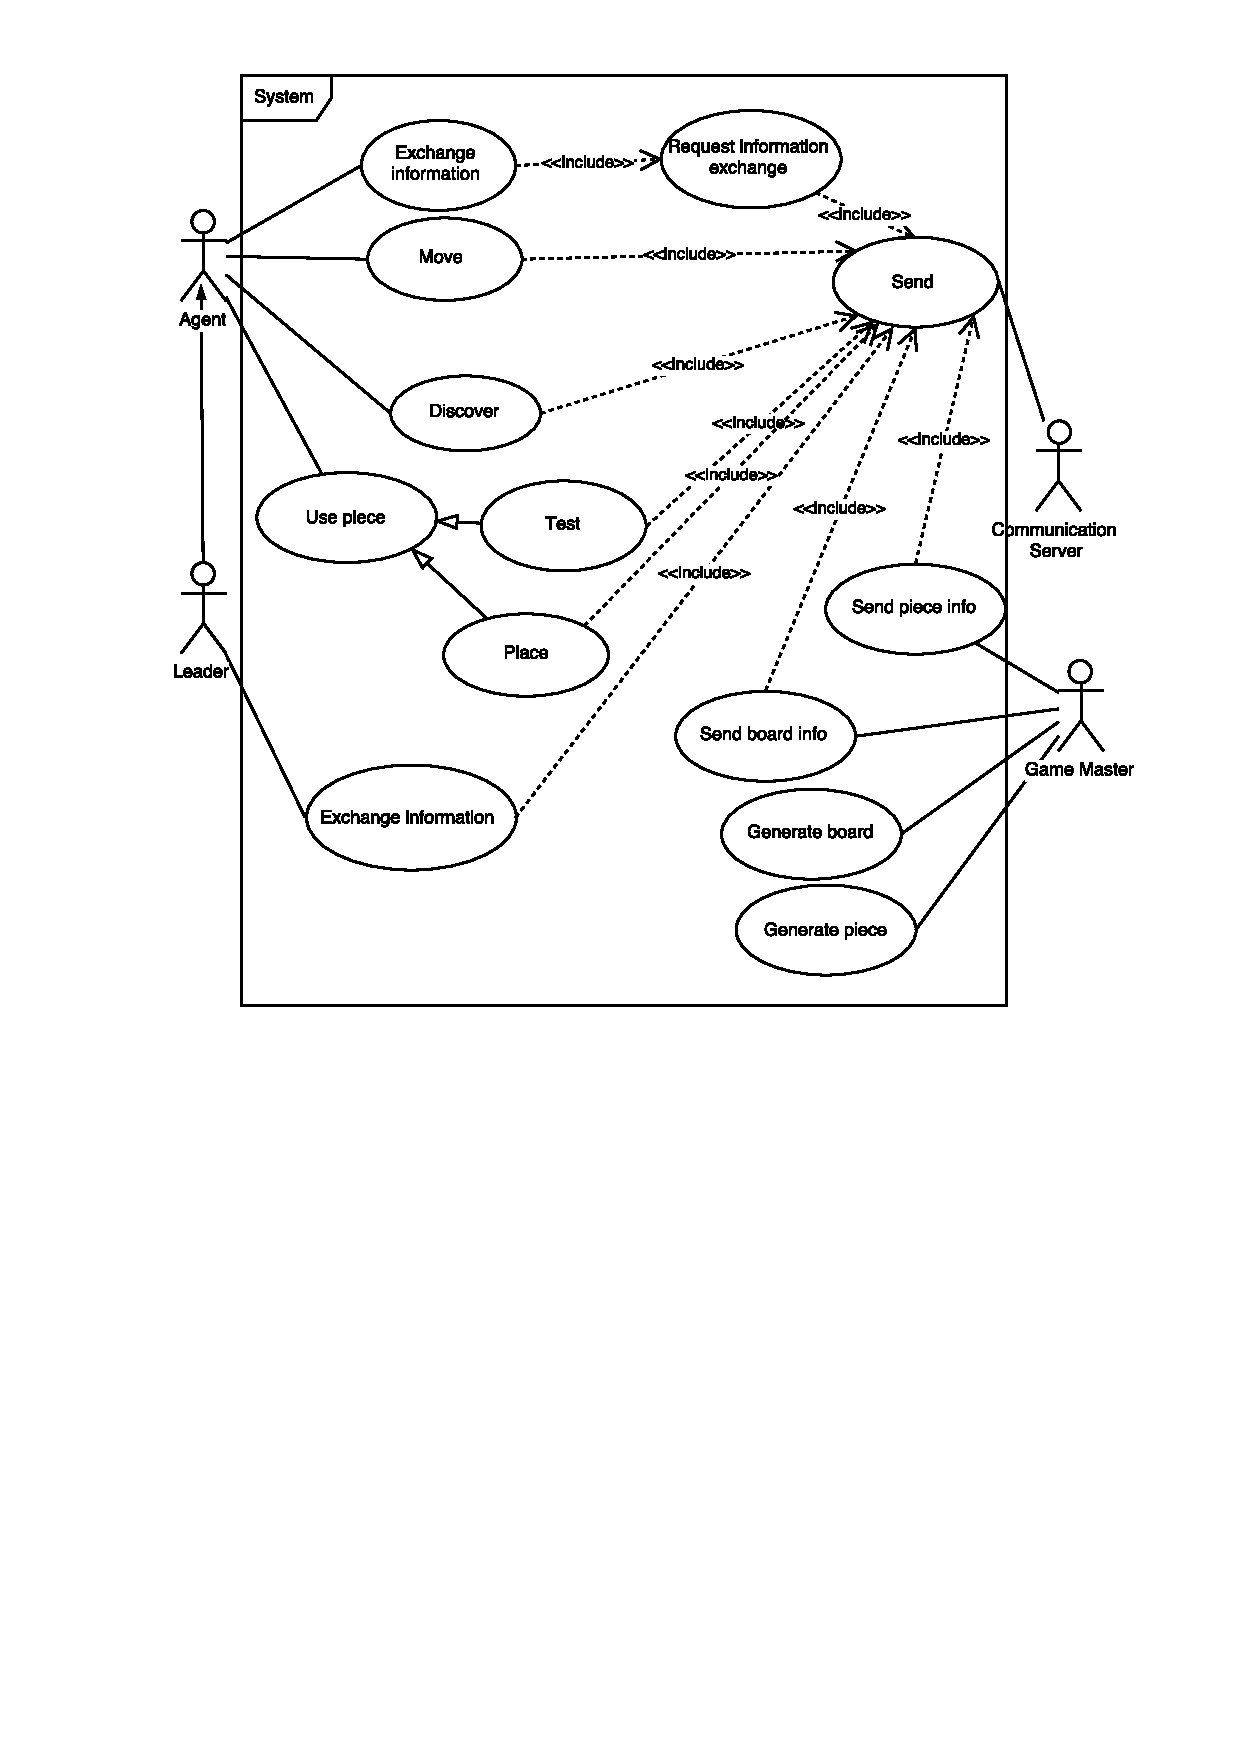
\includegraphics[scale=0.8]{./gameProjectUseCase_corrected}
%\captionof{figure}{Use Case'y game project}
%\end{figure}	
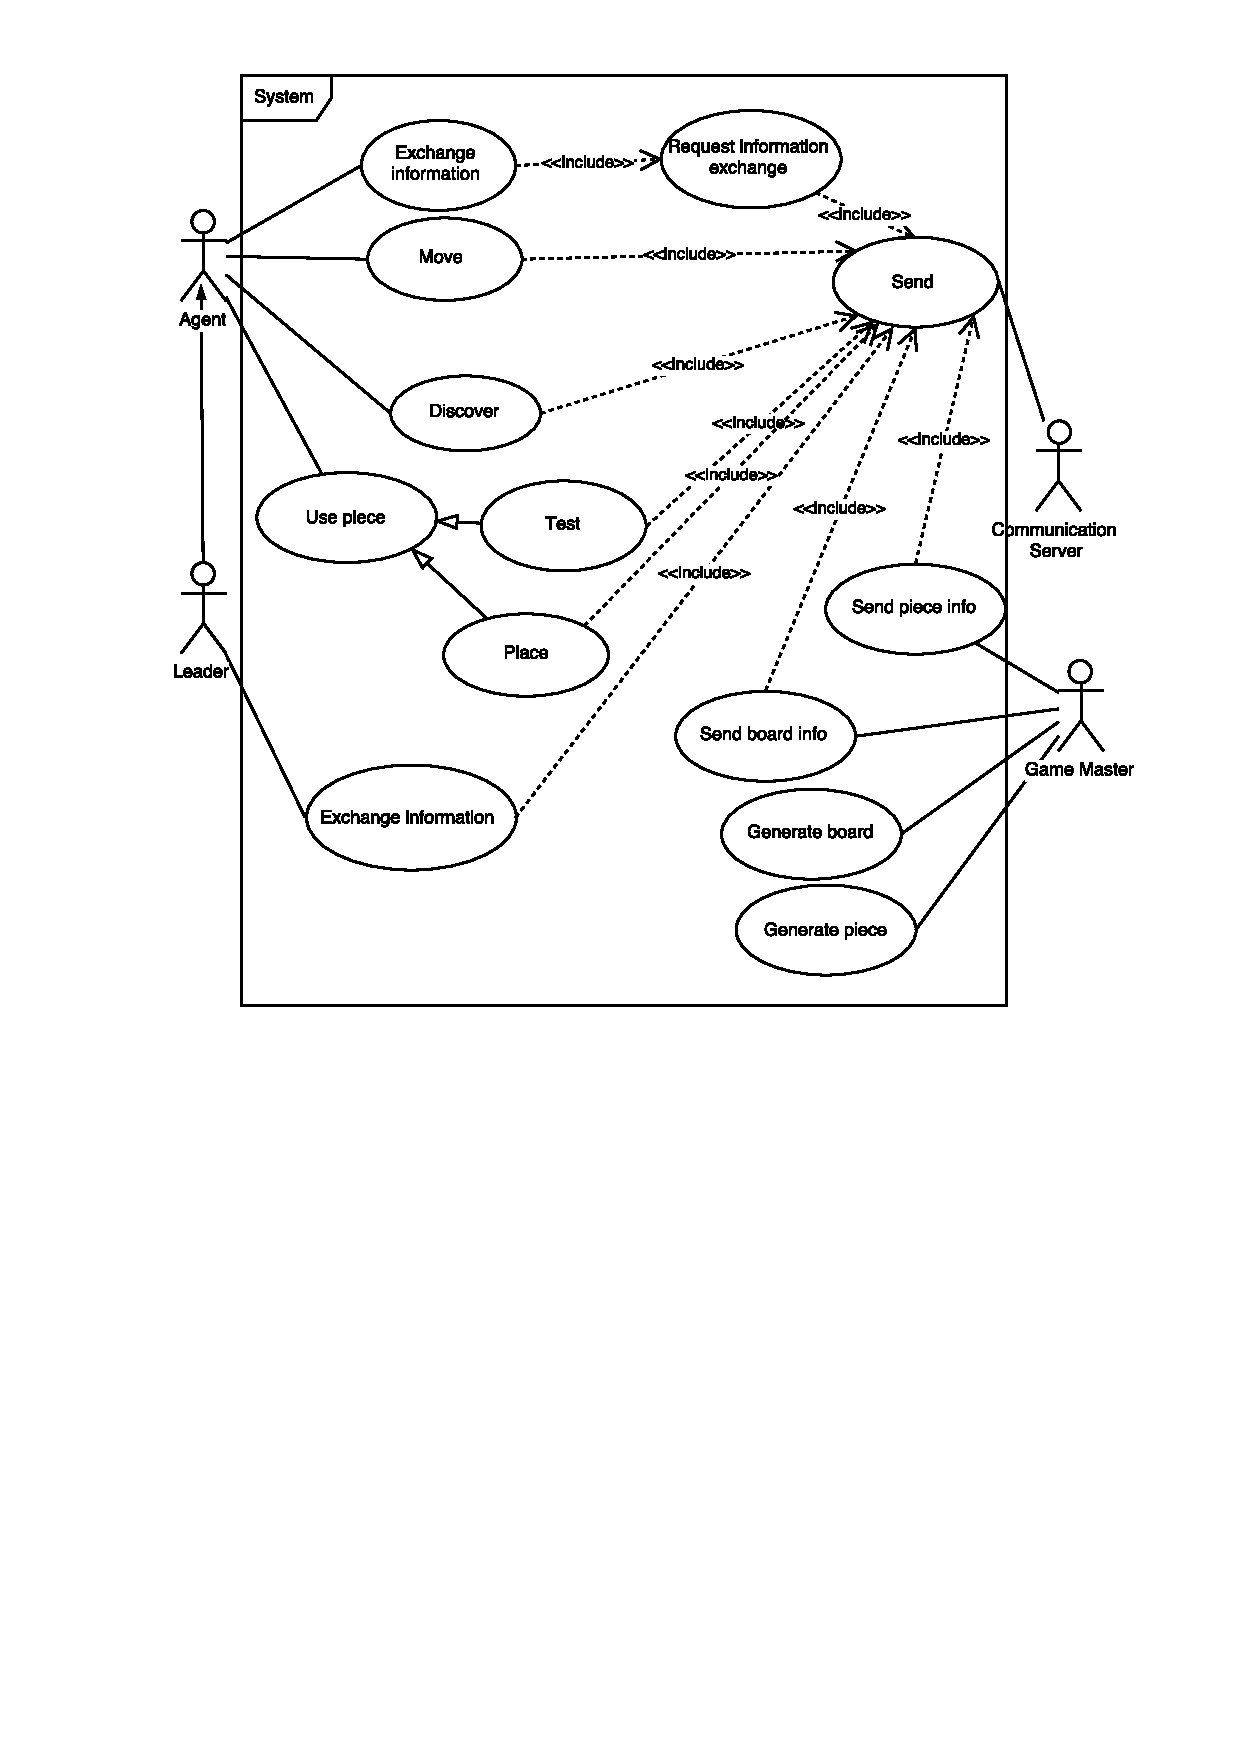
\includepdf[pages={1}]{./gameProjectUseCase_corrected.pdf}
	
	
%	\section{Architektura}


%	\begin{landscape}
%		\begin{figure}[htbp!]
%		\centering
%		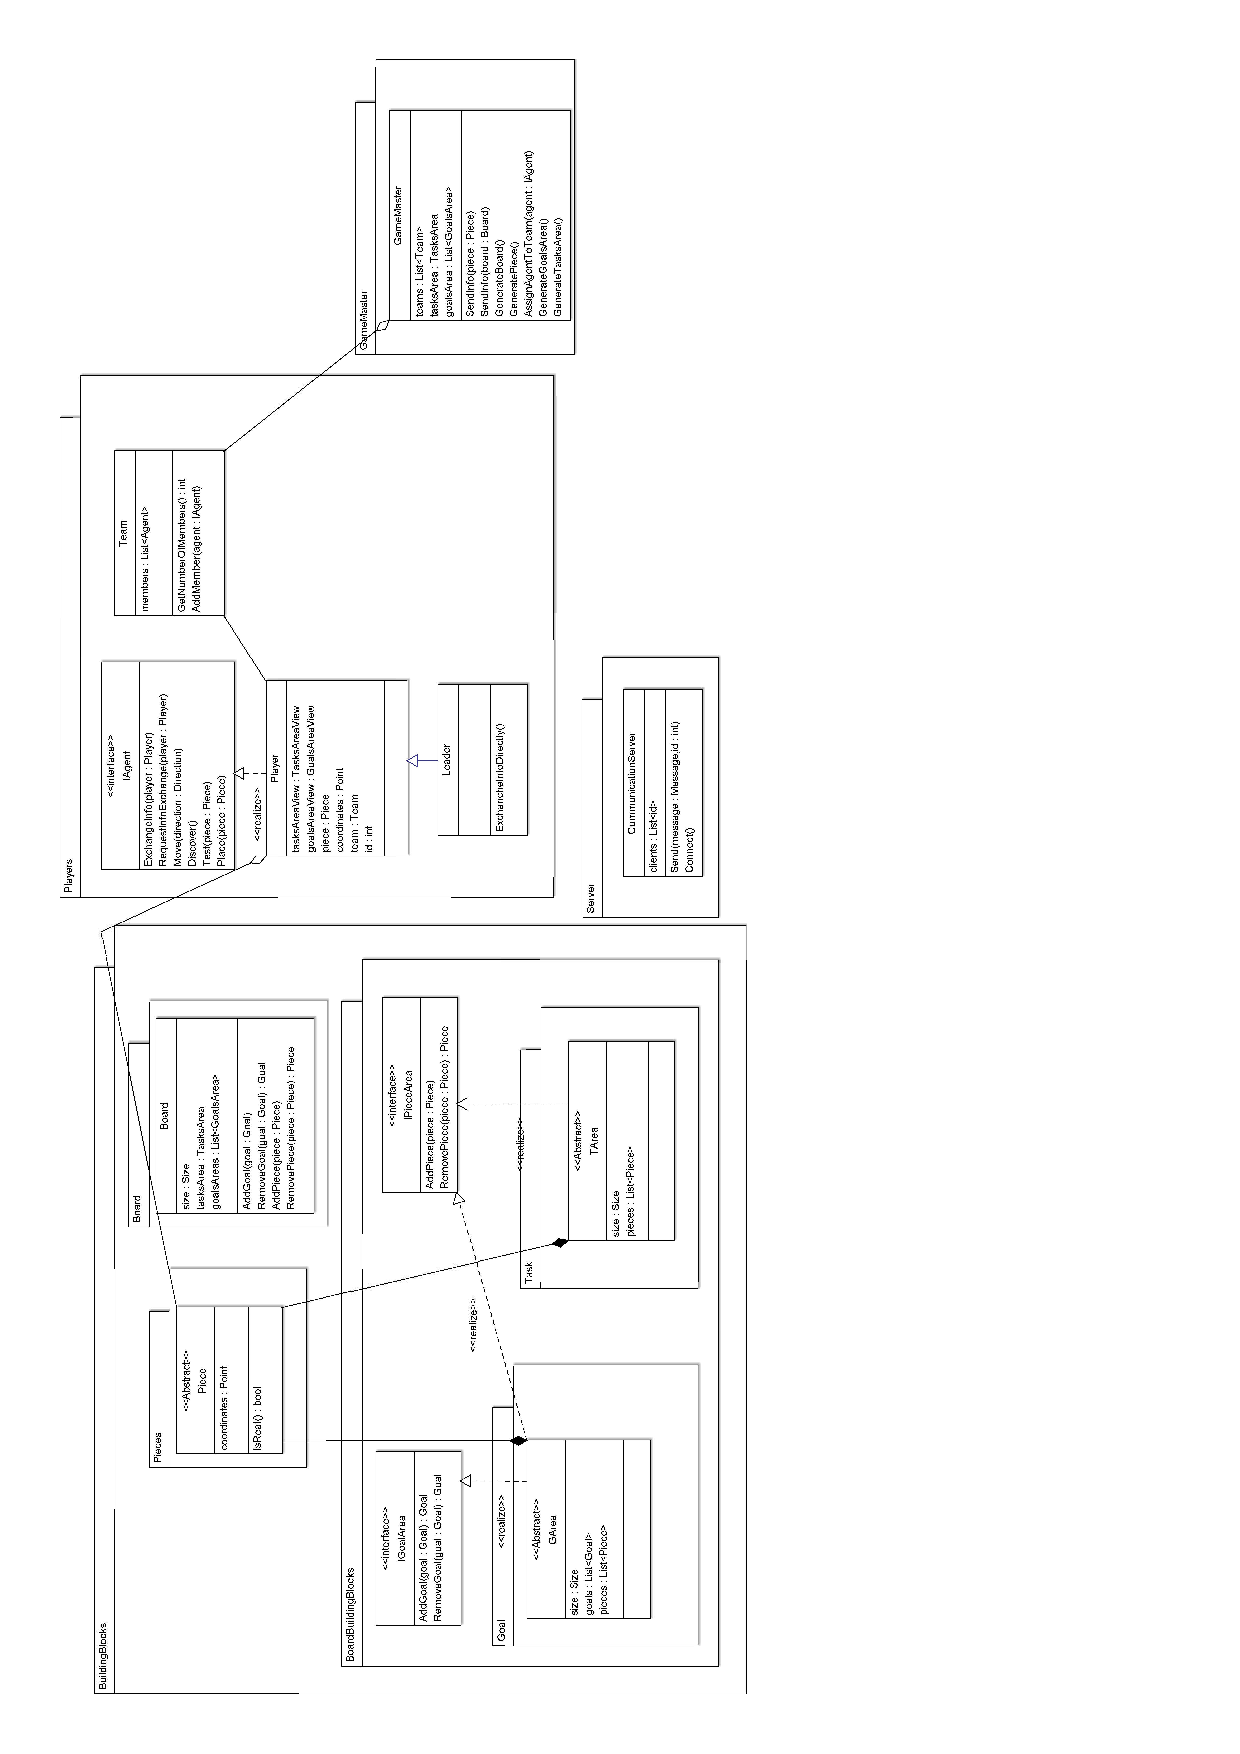
\includegraphics[scale=0.45]{./Class_Diagram}
%		\captionof{figure}{Architektura projektu}
%		\end{figure}	
%	\end{landscape}	

%shitty code, but it works :D
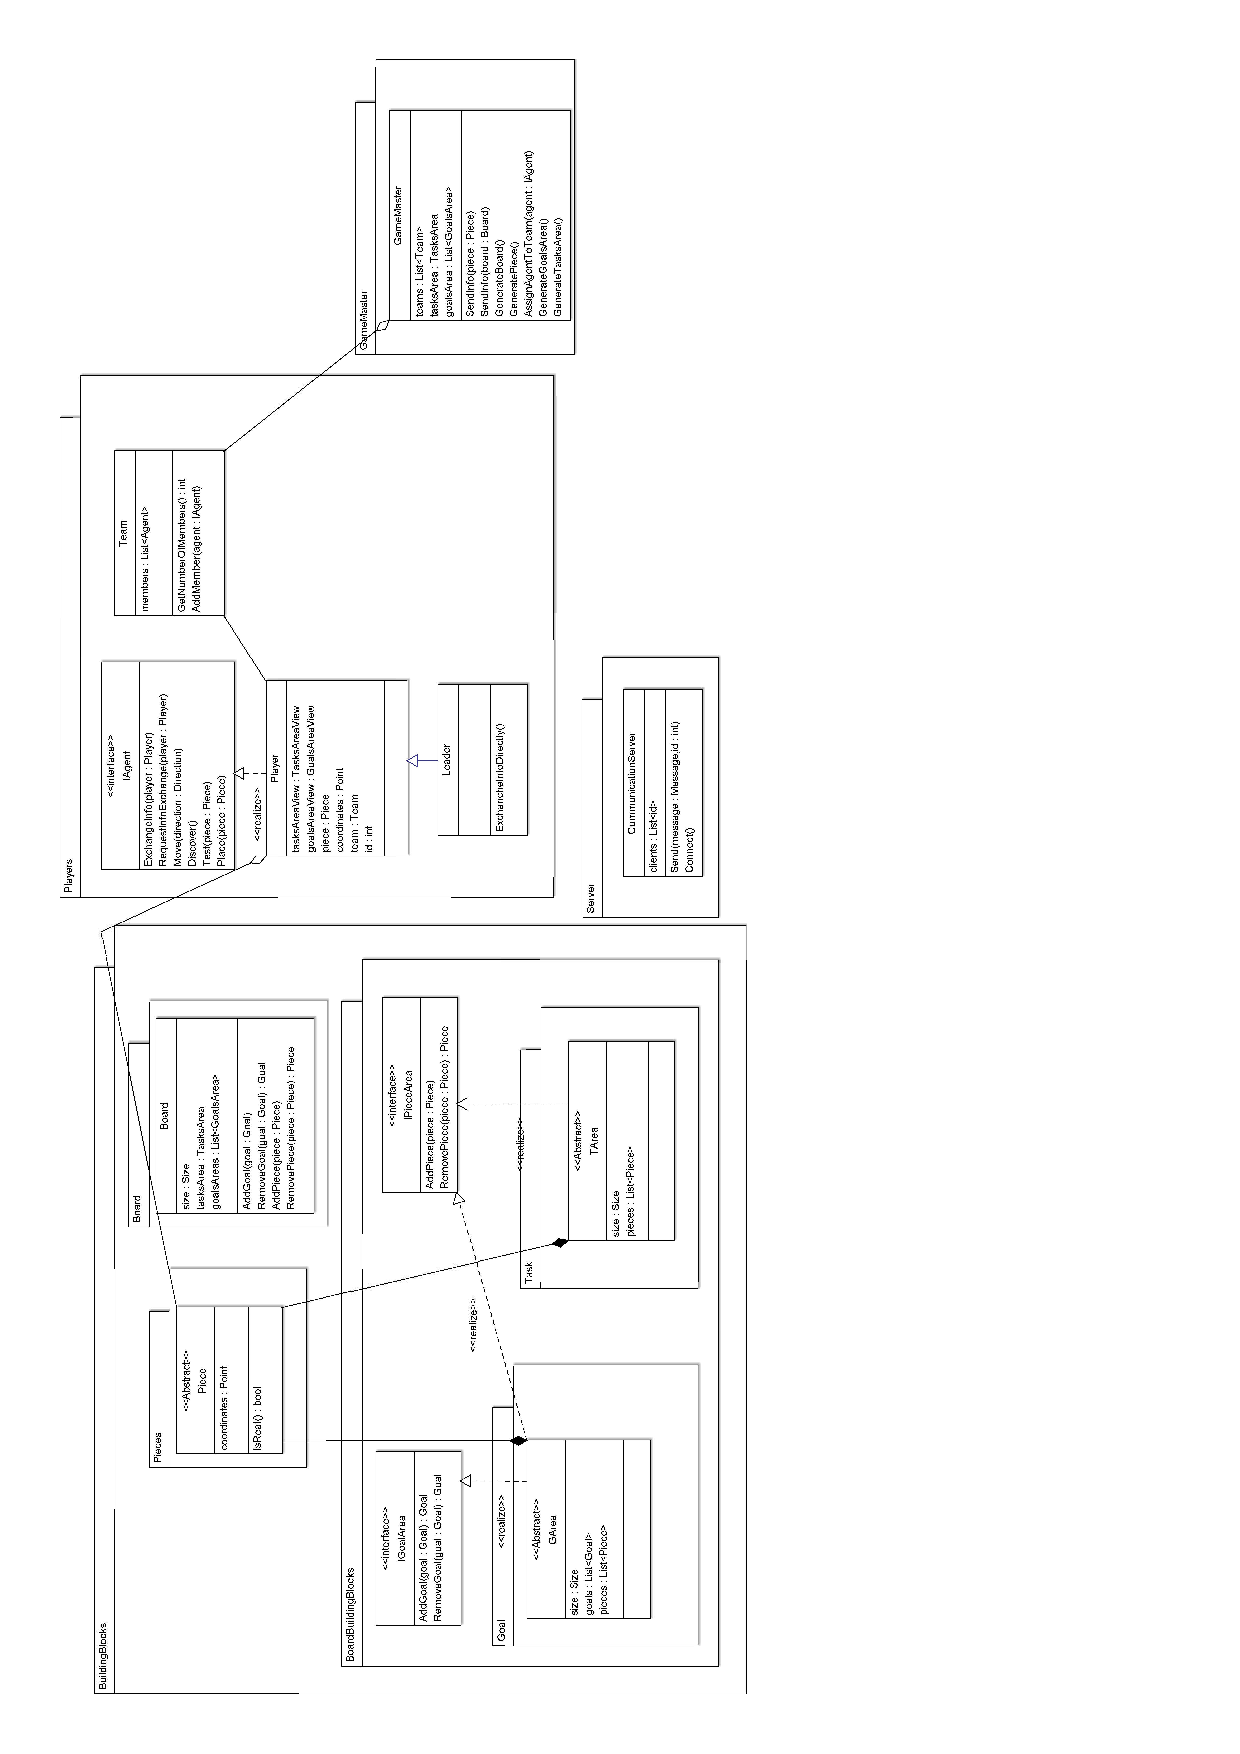
\includepdf[pages={1}]{./Class_Diagram.pdf}


	Dla przejrzystości architektury zostały pominięte po dwie klasy dziedziczące odpowiednio po GArea oraz TArea, odpowidają one za widok goal area oraz task area oraz dwie pozostałe reprezentujące task area oraz goal area.
	
	
\end{document}